\begin{frame}[fragile]{Proposed Method: K-Graph} 
\begin{block}{Knowledge Graph (K-Graph)}
    \begin{itemize}
      \item Store object's class
      \item Store action feedback
      \item Testing phase and converging phase
      \item Suggest actions
    \end{itemize}
  \end{block}
\end{frame}

\begin{frame}[fragile]{Proposed Method: K-Graph} 
  \begin{center}
    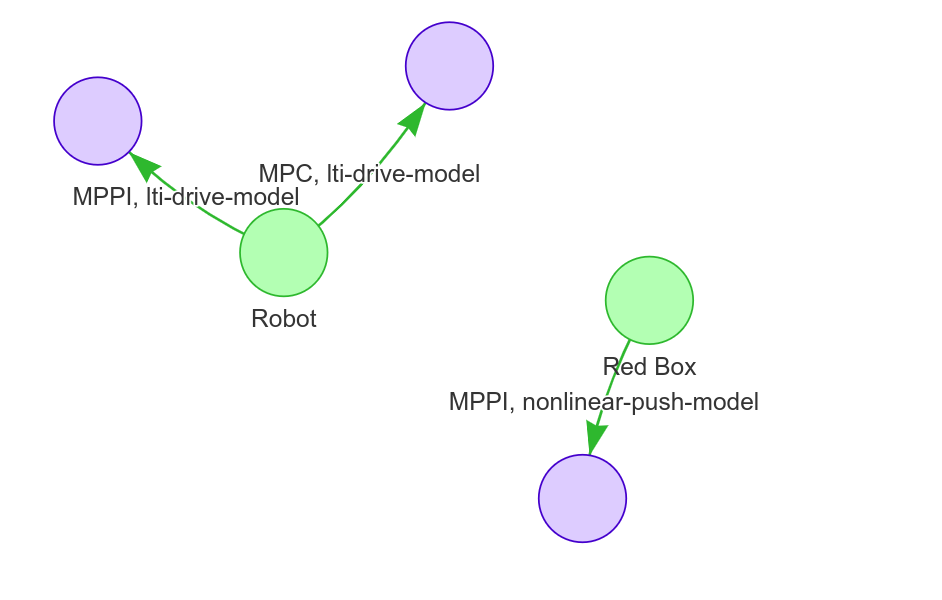
\includegraphics[height=0.9\textheight]{figures/proposed_method/kgraph_testing_phase}
  \end{center}
\end{frame}

\begin{frame}[fragile]{Proposed Method: K-Graph} 
  \begin{center}
    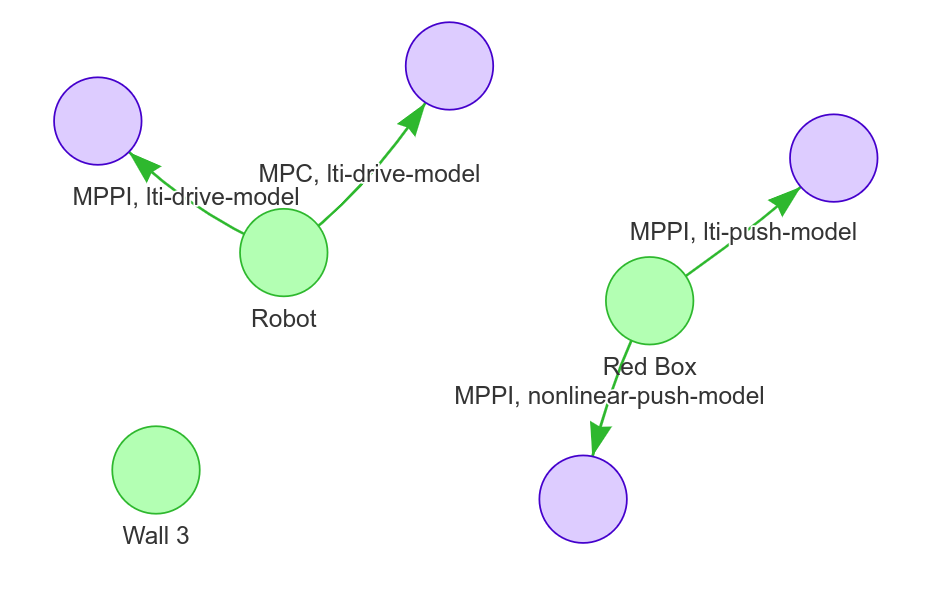
\includegraphics[height=0.9\textheight]{figures/proposed_method/kgraph_converging_phase}
  \end{center}
\end{frame}

% \begin{frame}[fragile]{Proposed Method: K-Graph} 
% Formally, a \textbf{\acl{k-graph}}, $\gls{k-graph} = \left\langle \gls{nodesK}, \gls{edgesK} \right\rangle $
% \\comprising $\gls{nodesK} = \{\gls{node}^{\mathit{center}}, \gls{node}^{\mathit{side}}\}$, \quad $\gls{edgesK} \in \{\gls{edge}_{(i,j)}| i \in \gls{nodesK}^\mathit{center}_\mathit{ids}, j \in \gls{nodesK}^\mathit{side}_\mathit{ids} \}$.\bs
% \end{frame}


\begin{frame}[fragile]{Proposed Method: K-Graph} 
  Action Feedback $\alpha$:\bs

  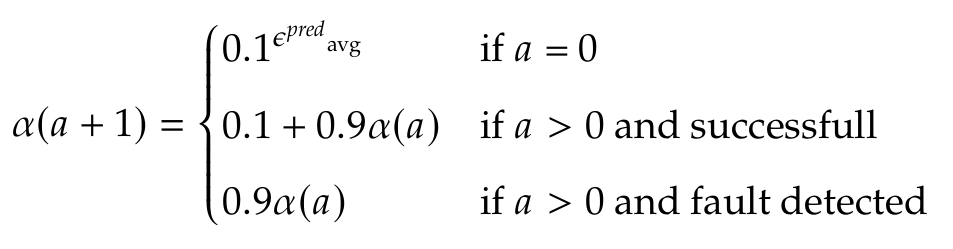
\includegraphics[width=0.7\textwidth]{figures/proposed_method/successfactor}\pause

  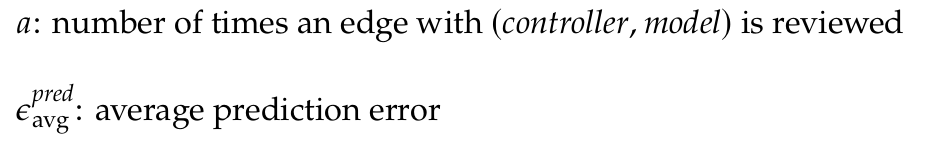
\includegraphics[width=0.8\textwidth]{figures/proposed_method/explain_successf}
\end{frame}
